\chapter{Result and Discussion} \label{chp:result_and_discussion}

The performance of GBM will be evaluated by means of a case study using the test dataset. The test dataset comprises journey data from the whole year of 2021. The first part will focus on performance evaluation of BBM, where the trained model will be used to predict the SOG. The second part focus on the power estimation method using Holtrop-Mennen method. The output of BBM, which is the ship SOG, will be fed to the WBM to estimate the power. For further clarity regarding the methodology, the following steps are taken which are based on the proposed methodology shown in \Cref{fig:flowchart_BBM} and \Cref{fig:flowchart_WBM}. For generation of the BBM, the steps taken are:

\begin{enumerate}
    \setlength\itemsep{0em}
    \item Dataset is loaded.
    \item Identify and remove any anomalies.
    \item Remove static and unneeded features.
    \item Apply speed threshold of 5 knots.
    \item Highly correlated features are combined/removed based on physical and statistical reasoning.
    \item Impute missing values using {\tt KNNImputer}.
    \item Split the dataset into training and testing.
    \item Train the model using the whole dataset with default hyperparameter.
    \item Evaluate model performance using k-fold cross-validation.
    \item Tune the model until the best model is obtained.
    \item For the case study, the best models will be used to predict the SOG using the test dataset.
\end{enumerate}

Subsequently, for FOC calculation, the following steps are taken:

\begin{enumerate}
    \setlength\itemsep{0em}
    \item The test dataset is split into seasonal data. Summer-Fall season and Winter-Spring season which correspond to data for 6 months respectively.
    \item SOG is converted to STW.
    \item Calculate calm water resistance $R_{CALM}$.
    \item Calculate added resistance due to wave $R_{AW}$.
    \item Calculate added resistance due to wind $R_{AA}$.
    \item Calculate total effective power $P_E$ using total resistance $R_{TOTAL}$.
    \item Calculate brake power $P_B$ from total efficiencies.
    \item Plot resulting regression line for Power-Speed curve from all models and actual case. 
    \item Calculate the FOC by considering the engine SFOC and operation time.
    \item Plot resulting regression line for FOC-Speed curve from all models and actual case.
    \item Evaluate the performance of the model generated from the regression lines.
\end{enumerate}

\section{Evaluation of BBM}\label{sec:BBM_tree_evaluate}

\subsection*{Model Training and Selection of Optimal Parameter}\label{sec:hpo_select_train}

As mentioned in \Cref{sec:BBM_modelling}. There are 2871 data points available for training. To help narrow the search range of the hyperparameters for the tree-based model, RMSE plots against different values of hyperparameters will be performed. This method was presented in \Cref{sec:hpo}. The hyperparameter will be iteratively tuned until the best model is obtained. The result of the optimal parameter is found in \Cref{tbl:hpo_optimal}. The model training is executed using \textbf{AMD Ryzen 7 2700X, Eight-Core Processor $@$ 3.7 GHz processor with 16384 MB installed RAM}.\\


\begin{table}[ht]
    \footnotesize
    \centering
    % \resizebox {\textwidth}{!}
    {\begin{tabular}{ p{0.1\linewidth} p{0.2\linewidth} p{0.3\linewidth}}
    \hline
    Model & Training time [s] & Optimal Hyperparameter \\
    \hline
    DTR & 0.044 & None \\
    $\text{DTR}_{OPT}$ & 0.021  & {\tt min\_samples\_split = 7}\\
    &&{\tt min\_samples\_leaf = 10}\\
    &&{\tt max\_features = 12}\\
    &&{\tt max\_depth = 8}\\
    RFR & 4.112 & None \\
    $\text{RFR}_{OPT}$ & 3.431  & {\tt min\_samples\_split = 2}\\
    &&{\tt min\_samples\_leaf = 1}\\
    &&{\tt max\_features = 10}\\
    &&{\tt max\_depth = 120}\\
    &&{\tt n\_estimators = 100}\\
    ETR & 0.944 & None \\
    $\text{ETR}_{OPT}$ & 4.390  & {\tt min\_samples\_split = 9}\\
    &&{\tt min\_samples\_leaf = 1}\\
    &&{\tt max\_features = 12}\\
    &&{\tt max\_depth = 120}\\
    &&{\tt n\_estimators = 800}\\
    MLR & 0.004  & None\\
    \hline
    \end{tabular}}
\caption{Optimal hyperparameter with training time of each model}\label{tbl:hpo_optimal}
\end{table}

With the default hyperparameter, RFR takes the longest training time followed by ETR and DTR. This is expected as RFR uses greedy algorithm i.e. it looks for the best possible feature when splitting the node. ETR takes significantly shorter time to train as ETR randomly select for features when splitting the node. DTR takes the shortest training time as it only generates a single tree. However, in the case of optimised model, ETR takes a longer time to train compared to RFR. This is caused by the number of trees in the optimised model which is controlled by the parameter {\tt n\_estimator}, the optimised ETR model has 800 trees in comparison to 100 trees of RFR. It is also observed that the training time of optimised DTR model is halved as pruning the tree resulted in a simpler model to train. \\

To further investigate the effect of hyperparameter optimisation, the learning curve of each tree-based model is plotted. For DTR, generated model with default parameter will result in a model that heavily overfits the training data, which is evident from the large gap between the training error and validation error which indicated a high variance as shown in \Cref{fig:learn_curve_DTR_RMSE}. Regularisation i.e. parameter tuning of the DTR model helps balance between bias and variance by trading bias for variance. This is observed from the substantial reduction in the gap between the training and validation error from \Cref{fig:learn_curve_DTR_RMSE}. Additionally, the learning curve indicates that the most notable improvement in model performance occurs until around 1000 data points. Beyond this point, the enhancement in model performance becomes less substantial.\\

\begin{figure}[h]
    \centering
        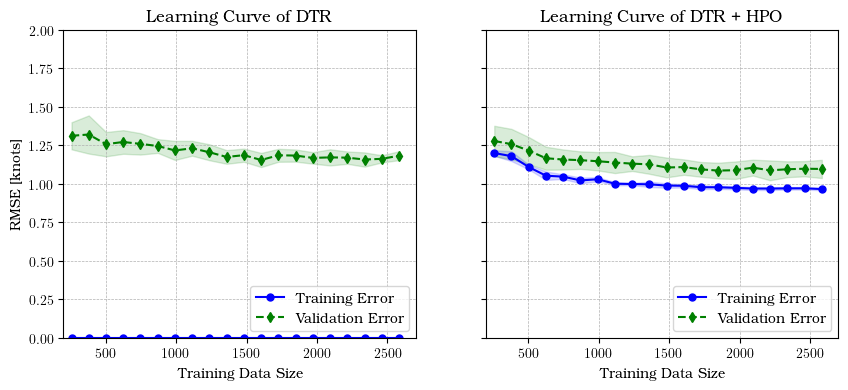
\includegraphics[width=.95\textwidth]{02_figures/learning_curve_dtr.png}
        \caption{Learning curve of DTR}
        \label{fig:learn_curve_DTR_RMSE}
\end{figure}

The process of hyperparameter tuning for the Random Forest Regressor (RFR) model did not show any significant improvement in model performance. This outcome aligns with the findings of  \bcitet{Kuhn.2013} and \bcitet{Hastie.2009} which was discussed in \Cref{sec:rf_theo}. The most notable improvement on model performance is observed until around 750 points, after which the model appears to reach a plateau. Furthermore, there is noticeable variance in the RFR model, which indicates that the model will have a slight tendency to overfit.

\begin{figure}[h]
    \centering
        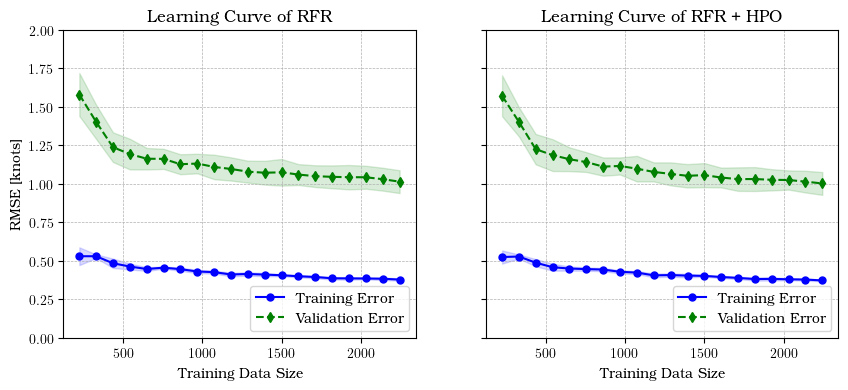
\includegraphics[width=.95\textwidth]{02_figures/learning_curve_rfr_rmse.png}
        \caption{Learning curve of RFR}
        \label{fig:learn_curve_RFR_RMSE}
\end{figure}

Hyperparameter tuning helps to reduce variance in the ETR model. But it does not have any major impact on model's performance. The ETR model reaches plateau beyond 1000 data points. Suggesting that adding more data points will not result in any significant increase in model performance.

\begin{figure}[h]
    \centering
        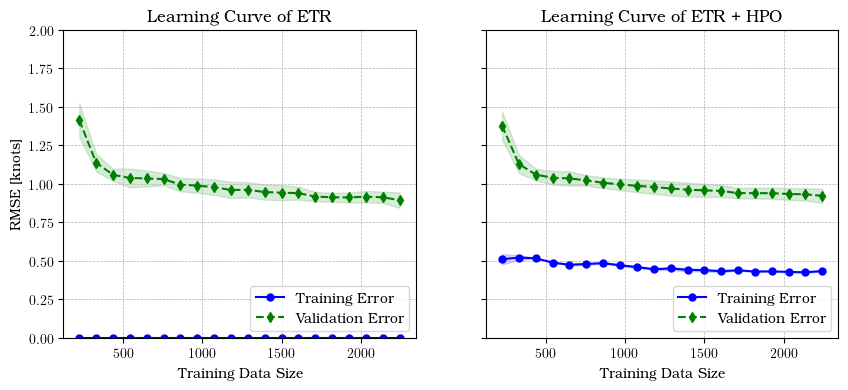
\includegraphics[width=.95\textwidth]{02_figures/learning_curve_etr_rmse.png}
        \caption{Learning curve of ETR}
        \label{fig:learn_curve_ETR_RMSE}
\end{figure}

In addition to the initial exploration in \Cref{sec:hpo}, it can be concluded that hyperparameter tuning for number of features and tree depth will have the biggest impact in affecting the model's performance. To improve training time, lower number of trees should be considered for RFR and ETR model.


\subsection*{Evaluation of trained model}\label{sec:BBM_model_eval}

The performance of the model is evaluated using the training dataset using 10-fold cross validation. This means that the training will be repeated 10 times using 9 of the folds as training dataset, the remaining fold will be used as validation dataset. The results from k-folding validation process is shown in \Cref{fig:train_boxplot_r2_rmse}. The inside (orange) line represents the median i.e. $50\%$ of the score in k-folding. The top and the bottom of the box correspond to the first i.e. $25\%$ and third quartile i.e. $75\%$ respectively. The whiskers represent the lowest data point within the 1.5 Interquartile Range (IQR) of the lowest quartile and the highest point of data within 1.5 IQR of the upper quartile. The mean is indicated by the (green) triangle. Data points beyond the whisker range is shown as hollow circle.\\

\begin{figure}[ht]
    \centering
    \subfigure[k-fold $R^2$ validation performance]{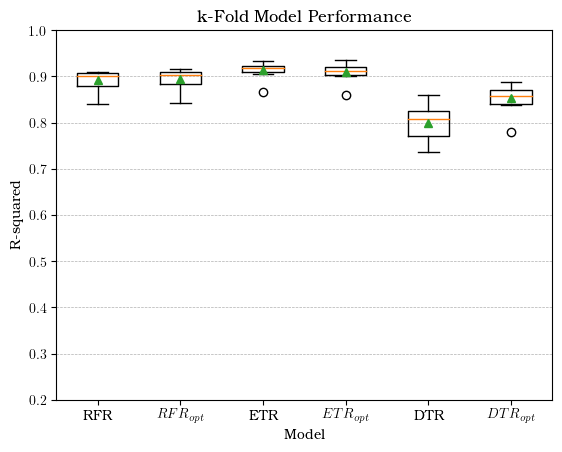
\includegraphics[width=0.49\textwidth]{02_figures/kfold_r2_opt.png}} 
    \subfigure[k-fold RMSE validation performance]{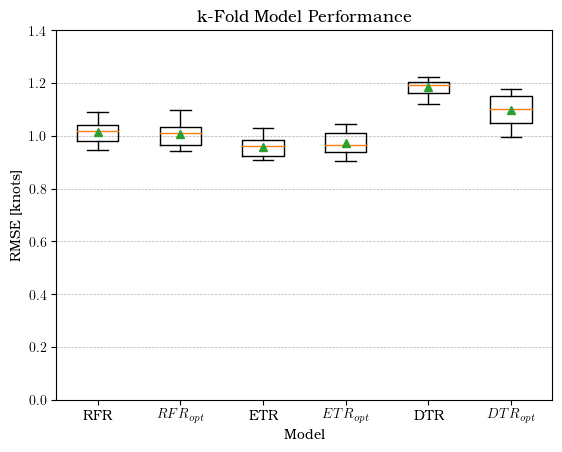
\includegraphics[width=0.49\textwidth]{02_figures/kfold_rmse_opt.png}}
    \caption{Box plots of different models with default and optimised parameter in k-folding for training dataset}
    \label{fig:train_boxplot_r2_rmse}
\end{figure}

The box plots indicated that ETR achieved the best performance, the model is able to achieve $R^2$ score of around $91\%$ and RMSE of around 0.96 knots. The model is also relatively stable, which is indicated by the narrow box plots. RFR also achieved similar performance, achieving $R^2$ score of about $89\%$ and RMSE of approximately 1.00 knots and slightly worse stability. This behaviour may be caused due to the high variance shown from the learning curves shown in \Cref{fig:learn_curve_RFR_RMSE} and \Cref{fig:learn_curve_ETR_RMSE}. This means that the model will have slight tendency to overfit.\\

DTR greatly benefits from regularisation, the model achieve an increase of about $5\%$ for the $R^2$ score and a reduction from about 1.2 knots to 1.1 knots for the RMSE. To summarise, all tree based models exhibited good performance, all models achieved good fit with mean/median $R^2$ scores above $80\%$. However, the RMSE is quite significant at range of 1.00 to 1.20 knots across the models. To put this into scale, the mean SOG of the training data is at 16.91 knots as shown in \Cref{tbl:dataset_descriptive_pretraining}.\\  